\section{FFS}
The product of this thesis is the Fejk File System (FFS) which uses online services to store the data but behaves like a mountable disk for the users. The file system will however be very basic and not support all functionalities that other systems do such as links. The reasoning is that these behaviours are not required for a useable system, and when comparing the system to distributed filesystems such as Google Drive, they often do not support his either.

Figure~\ref{fig:ffs_inode_diag} describes the basic outline of FFS which is based on the idea of inode filsystems. Instead of an inode pointing to specific blocks in a disk, the inodes of FFS will instead point keep track of the id numbers of the posts to online services where the file is located. 

\begin{figure}[!ht]
	\begin{center}
	  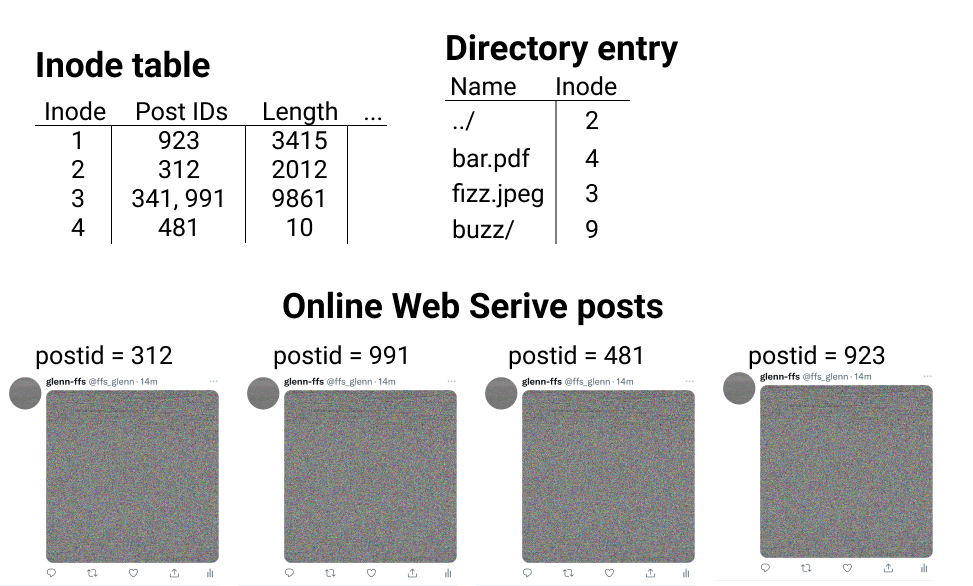
\includegraphics[width=0.8\textwidth]{figures/ffs_inode_diagram.png}
	\end{center}
	\caption{Basic structure of FFS inode-based structure}
	\label{fig:ffs_inode_diag}
\end{figure}

